\documentclass[final]{article}

\usepackage{neurips_2025}

\usepackage[utf8]{inputenc}
\usepackage[T1]{fontenc}
\usepackage{hyperref}
\usepackage{url}
\usepackage{booktabs}
\usepackage{amsfonts}
\usepackage{nicefrac}
\usepackage{microtype}
\usepackage{xcolor}
\usepackage{amsmath}
\usepackage{graphicx}
\usepackage{subcaption}
\usepackage{multirow}
\usepackage{enumitem}

\graphicspath{{../temporal/figures/}{../enhanced/figures/}{../figures/}{../img/}}

\title{SleepStageNet: Deep Learning for Automated Sleep Stage Classification}

\author{%
  Shrinivas Acharya \\
  % University of Washington \\
  \texttt{acharyas@cs.washington.edu} \\
  \And
  Manish Das \\
  % University of Washington \\
  \texttt{manishuw@cs.washington.edu} \\
  \AND
  Nithin Balachandran \\
  % University of Washington \\
  \texttt{nibalach@cs.washington.edu} \\
  \And
  Regith Lingesh \\
  % University of Washington \\
  \texttt{rlingesh@cs.washington.edu} \\
  \And
  Thangakumar Dhanasekaran \\
  % University of Washington \\
  \texttt{tdhana@cs.washington.edu} \\
}

\begin{document}

\maketitle

\begin{abstract}
Automated sleep staging from raw electroencephalography (EEG) signals promises to reduce the cost and subjectivity of manual polysomnography scoring, which currently requires 2--4 hours of expert effort per overnight recording. We present a systematic comparison of three progressively complex architectures for 5-class sleep stage classification on the Sleep-EDF v1 dataset: (1)~a dual-path multi-scale CNN baseline inspired by DeepSleepNet-Lite, (2)~the same CNN backbone augmented with a two-layer bidirectional LSTM for temporal context modeling, and (3)~a CNN--Conformer hybrid that replaces the recurrent layer with Conformer blocks combining multi-head self-attention and depthwise convolution. All models are evaluated under an identical 20-fold leave-one-subject-out cross-validation protocol. The CNN+BiLSTM achieves the best performance with 83.9\% accuracy, macro F1 of 0.79, and Cohen's $\kappa$ of 0.778---approaching the lower bound of human inter-scorer agreement ($\kappa \approx 0.75$--$0.85$). Notably, the BiLSTM outperforms the Conformer across all metrics despite having fewer parameters, suggesting that recurrent inductive biases are preferable to attention mechanisms on small sequential EEG datasets. Our results confirm that temporal context modeling is the single most impactful architectural choice, yielding a 3 percentage-point accuracy improvement and a 17.7\% relative gain on the challenging N1 stage.
\end{abstract}

%==============================================================================
\section{Introduction}
%==============================================================================

Sleep disorders affect an estimated 50--70 million Americans, yet diagnosis remains bottlenecked by the manual scoring of polysomnography (PSG) recordings~\cite{Berry2012}. A trained technician examines each 30-second epoch and assigns one of five stages---Wake~(W), N1, N2, N3, and REM---per AASM guidelines. With 800--1,000 epochs per night, this takes 2--4 hours per recording and exhibits inter-scorer disagreement with Cohen's $\kappa$ typically 0.75--0.85~\cite{Rosenberg2013}.

Deep learning has shown strong potential. DeepSleepNet~\cite{Supratak2017} introduced a dual-path CNN with a BiLSTM for raw single-channel EEG. U-Sleep~\cite{Perslev2021} demonstrated cross-dataset generalization. AttnSleep~\cite{Eldele2021} applied attention mechanisms, and SleepTransformer~\cite{Phan2022} used epoch-level and sequence-level transformer blocks. Despite these advances, a key question remains: \emph{given the same feature extraction backbone, does recurrent or attention-based temporal modeling yield better performance on small EEG datasets?}

We address this through a controlled comparison of three architectures sharing a common multi-scale CNN backbone, differing only in temporal modeling: no temporal modeling (baseline), a two-layer BiLSTM, and a three-block Conformer---all evaluated under identical 20-fold LOSO-CV on Sleep-EDF v1.

Our contributions are: (1)~a systematic comparison showing temporal context is the dominant factor (+3 pp accuracy over baseline); (2)~evidence that BiLSTM outperforms the Conformer on small EEG datasets, achieving $\kappa = 0.778$; and (3)~per-class analysis revealing temporal models most benefit stages with ambiguous spectral signatures (N1, Wake, REM). Our code is publicly available~\cite{SleepStageNetRepo}.

%==============================================================================
\section{Related Work}
%==============================================================================

\paragraph{From hand-crafted features to end-to-end learning.}
Early automated sleep staging relied on hand-crafted features---spectral band powers, Hjorth parameters, and wavelet coefficients---fed into SVMs or random forests. These approaches required expert feature engineering and generalized poorly across recording setups. The shift to end-to-end deep learning, where raw EEG is input directly to a neural network, eliminated this bottleneck and enabled models to discover discriminative features automatically.

\paragraph{CNN-based methods.}
DeepSleepNet~\cite{Supratak2017} pioneered a dual-path CNN with small filters ($\sim$0.5\,s) for high-frequency features and large filters ($\sim$4\,s) for slow waves, followed by a BiLSTM. DeepSleepNet-Lite~\cite{Fiorillo2019} simplified this to reduce computational cost while preserving the dual-path concept---demonstrating that much of the performance could be retained with fewer parameters. Our baseline adopts this philosophy.

\paragraph{Temporal and attention-based methods.}
LSTMs~\cite{Hochreiter1997} and bidirectional variants have been widely used for modeling sleep stage transitions, as they naturally encode the sequential nature of overnight recordings. More recently, AttnSleep~\cite{Eldele2021} applied multi-head attention over CNN features, allowing the model to weight distant epochs dynamically. SleepTransformer~\cite{Phan2022} introduced a dual-granularity approach with epoch-level transformers for intra-epoch feature extraction and sequence-level transformers for inter-epoch dependencies. The Conformer~\cite{Gulati2020}, originally developed for speech recognition, uniquely combines self-attention (for global context) with depthwise convolution (for local patterns). We adapt it for EEG epoch sequences, hypothesizing that this dual mechanism may benefit sleep staging where both global sleep structure and local transition smoothness matter.

\paragraph{Training techniques for imbalanced data.}
Focal loss~\cite{Lin2017} down-weights easy examples to focus on hard cases, which is particularly relevant for underrepresented stages like N1. Mixup interpolates training pairs to produce smoother decision boundaries and has been shown to improve generalization on small datasets. We combine these with a three-stage training pipeline and cosine annealing with warmup.

\paragraph{Evaluation protocols.}
A critical but often overlooked factor in comparing sleep staging methods is the evaluation protocol. Many studies use random 80/20 train/test splits or k-fold cross-validation without ensuring subject independence---meaning epochs from the same subject can appear in both training and testing, inflating reported accuracy by 3--5 percentage points. Leave-one-subject-out (LOSO) cross-validation, which we employ, is the most stringent protocol: it guarantees that the model has never seen any data from the test subject during training. This better reflects real-world deployment, where the model must generalize to entirely new patients.

%==============================================================================
\section{Dataset}
%==============================================================================

We use the \textbf{Sleep-EDF v1} dataset from PhysioNet~\cite{SleepEDF2018}\footnote{\url{https://physionet.org/content/sleep-edfx/1.0.0/}}: 39 whole-night PSG recordings from 20 healthy subjects, providing the Fpz-Cz EEG channel at 100\,Hz with expert AASM annotations~\cite{Berry2012} for each 30-second epoch (3,000 samples).

The dataset contains 42,308 epochs with severe class imbalance (Figure~\ref{fig:class_dist}): N2 dominates at 42.1\%, while the transitional N1 stage comprises only 6.6\%---a 6.4:1 ratio. This makes accuracy misleading (a majority-class classifier achieves 42\%) and motivates macro F1 as our primary metric.

\begin{figure}[t]
  \centering
  
\includegraphics[width=0.60\columnwidth]{class_distribution.png}
  \caption{Sleep stage distribution in Sleep-EDF v1 (42,308 epochs, 39 recordings). N2 dominates at 42.1\%; the transitional N1 stage is only 6.6\%.}
  \label{fig:class_dist}
\end{figure}

%==============================================================================
\section{Methods}
%==============================================================================

We develop three architectures of increasing complexity, all sharing a multi-scale CNN feature extractor and differing in temporal context modeling. Our progression is motivated by a key clinical insight: sleep technicians never score an epoch in isolation---they examine the surrounding context to resolve ambiguities. Our models formalize this intuition at increasing levels of sophistication.

%--------------------------------------
\subsection{Multi-Scale CNN Backbone}
\label{sec:cnn_backbone}
%--------------------------------------

EEG signals contain diagnostically relevant features at vastly different time scales. Sleep spindles (12--14\,Hz) and K-complexes are transient events lasting $\sim$0.5--1\,s, while slow-wave/delta activity (0.5--2\,Hz) unfolds over 2--4\,s. A single convolutional filter size cannot efficiently capture both. Inspired by DeepSleepNet~\cite{Supratak2017} and DeepSleepNet-Lite~\cite{Fiorillo2019, DSLOriginalRepo}, we use two parallel paths operating at different temporal resolutions:

\textbf{Path~A (fine-grained, $\sim$0.5\,s)} targets high-frequency features: Conv1d($C_{\text{in}} \!\to\! 32$, $k\!=\!50$, $s\!=\!6$) $\to$ BN $\to$ ReLU $\to$ MaxPool(8) $\to$ three Conv1d($\to$64, $k\!=\!8$) blocks with BN+ReLU $\to$ MaxPool(4) $\to$ AdaptiveAvgPool(1) $\to$ 64-dim. At 100\,Hz, a kernel of size 50 spans 0.5\,s---well-matched to spindle duration.

\textbf{Path~B (coarse, $\sim$4\,s)} targets low-frequency features: Conv1d($C_{\text{in}} \!\to\! 32$, $k\!=\!400$, $s\!=\!50$) $\to$ BN $\to$ ReLU $\to$ MaxPool(4) $\to$ three Conv1d($\to$64, $k\!=\!6$) blocks $\to$ MaxPool(2) $\to$ AdaptiveAvgPool(1) $\to$ 64-dim. A kernel of 400 spans 4\,s, covering full cycles of delta waves that characterize N3 deep sleep.

The two 64-dim outputs are concatenated, passed through dropout~(0.5), and projected to a 128-dimensional feature vector. This design mirrors how an EEG specialist reads recordings: first scanning for fast transient events (spindles, K-complexes), then assessing the slower background rhythm. The backbone is shared across temporal models and applied independently to each epoch.

%--------------------------------------
\subsection{Model~1: CNN-Only Baseline}
%--------------------------------------

The baseline concatenates three consecutive 30-second epochs into a 90-second window (9,000 samples) and passes it through a dual-path CNN following the original DeepSleepNet-Lite design~\cite{Fiorillo2019} in TensorFlow, using 64/128 channel filters without adaptive pooling ($\sim$648K parameters). Training uses Adam (lr~$= 10^{-4}$), batch size 100, 100 epochs with early stopping (patience~50), and minority-class oversampling.

This model provides limited temporal context through the concatenated window but treats each 90-second segment as a monolithic input---it cannot explicitly reason about \emph{which features came from which epoch} or model the sequential structure of sleep.

%--------------------------------------
\subsection{Model~2: CNN + BiLSTM}
\label{sec:bilstm}
%--------------------------------------

Sleep stages follow a biological progression: subjects typically cycle through Wake $\to$ N1 $\to$ N2 $\to$ N3 $\to$ N2 $\to$ REM $\to$ Wake in $\sim$90-minute cycles, with deep sleep dominating early in the night and REM lengthening toward morning. A CNN that classifies each epoch independently cannot leverage these transition patterns. The key insight behind our temporal model is that \emph{knowing what came before and after an epoch dramatically reduces ambiguity}---for instance, an epoch with mixed theta and alpha activity is likely N1 if preceded by Wake epochs and followed by N2, but likely REM if preceded by N2 and followed by Wake.

We formalize this with a bidirectional LSTM~\cite{Hochreiter1997}. Each epoch is first processed independently through the shared CNN backbone (Section~\ref{sec:cnn_backbone}) to obtain a 128-dim feature vector. A sequence of $L = 11$ consecutive features ($\pm$5 epochs, i.e., $\pm$2.5 minutes of context) is then passed to a \textbf{two-layer BiLSTM} with hidden size 128 per direction, producing a 256-dim output per timestep. The forward LSTM reads the sequence left-to-right (past $\to$ present), while the backward LSTM reads right-to-left (future $\to$ present), and their outputs are concatenated at each position. The center epoch (position~5) receives the richest context---full bidirectional information from all 10 surrounding epochs---and is classified through dropout~(0.3) and a linear layer to 5 classes.

Using two stacked LSTM layers enables hierarchical temporal abstraction: the first layer captures local patterns (e.g., N2$\to$N3 transitions), while the second layer can model longer-range dependencies (e.g., REM cycle timing). The model has $\sim$851K parameters.

%--------------------------------------
\subsection{Model~3: CNN + Conformer}
\label{sec:conformer}
%--------------------------------------

While the BiLSTM processes epochs sequentially, its ability to relate distant positions depends on information propagating through the hidden state chain. The Conformer~\cite{Gulati2020} addresses this differently: self-attention provides \emph{direct} connections between any two epochs (capturing global patterns like ``this REM epoch 4 minutes ago predicts another REM epoch now''), while depthwise convolution captures \emph{local} smoothness (adjacent epochs tend to share the same stage).

This model replaces the BiLSTM with \textbf{three Conformer blocks}, each using the Macaron-style architecture: (1)~half-step FFN (Linear 128$\to$512$\to$128, GELU, 0.5$\times$ residual); (2)~multi-head self-attention (4 heads, $d_k = 32$); (3)~convolution module (pointwise conv $\to$ GLU $\to$ depthwise conv $k\!=\!7$ $\to$ BN $\to$ GELU $\to$ pointwise conv); (4)~half-step FFN; (5)~final LayerNorm.

Learnable positional encoding is added before the Conformer blocks, as it outperforms fixed sinusoidal encoding for short sequences ($L = 11$). The model uses focal loss~\cite{Lin2017} with $\gamma = 1.5$ to focus on hard examples (particularly N1, the rarest and most ambiguous stage). It has $\sim$1.34M parameters.

%--------------------------------------
\subsection{Training Strategy}
\label{sec:training}
%--------------------------------------

Jointly training a CNN and temporal layer from scratch is unstable: the temporal layer receives uninformative features from an untrained CNN, preventing meaningful gradient signal. Both temporal models therefore use a \textbf{three-stage training pipeline}: \textbf{Stage~1}---pretrain the CNN as a single-epoch classifier (AdamW, lr~$= 10^{-3}$, up to 50 epochs); \textbf{Stage~2}---freeze CNN weights and train only the temporal layers on $L = 11$ sequences (up to 50 epochs); \textbf{Stage~3}---unfreeze all parameters and fine-tune end-to-end with 10$\times$ reduced learning rate (up to 30 epochs).

\paragraph{Regularization.} We employ Mixup ($\alpha = 0.1$, 50\% of batches), label smoothing (0.05), EEG-specific augmentation (time shift $\pm$50 samples, amplitude scaling $\pm$10\%, Gaussian noise), cosine annealing with 3-epoch warmup, and gradient clipping (max norm 1.0). Class imbalance is addressed via inverse class-frequency weighting.

Table~\ref{tab:hyperparams} summarizes the hyperparameters.

\begin{table}[t]
\caption{Hyperparameter comparison across the three models.}
\label{tab:hyperparams}
\centering
\small
\begin{tabular}{lccc}
\toprule
\textbf{Hyperparameter} & \textbf{Baseline} & \textbf{CNN+BiLSTM} & \textbf{Conformer} \\
\midrule
Framework        & TensorFlow   & PyTorch     & PyTorch \\
Sequence length  & 3 (concat)   & 11          & 11 \\
Batch size       & 100          & 32          & 32 \\
Learning rate    & $10^{-4}$    & $5 \times 10^{-4}$ & $3 \times 10^{-4}$ \\
Optimizer        & Adam         & AdamW       & AdamW \\
Loss function    & Cross-entropy & Cross-entropy & Focal ($\gamma\!=\!1.5$) \\
Mixup $\alpha$   & ---          & 0.1         & 0.1 \\
Label smoothing  & 0            & 0.05        & 0.05 \\
Patience         & 50           & 15          & 20 \\
Parameters       & $\sim$648K   & $\sim$851K  & $\sim$1.34M \\
\bottomrule
\end{tabular}
\end{table}

%--------------------------------------
\subsection{Evaluation}
%--------------------------------------

We use \textbf{20-fold leave-one-subject-out cross-validation} (LOSO-CV): each fold holds out one subject for testing, with the remaining 19 split into training (15) and validation (4). Sequences never cross recording boundaries. We report accuracy, \textbf{macro F1} (primary---treats all classes equally), Cohen's $\kappa$ (the clinical standard, correcting for chance agreement), and per-class F1. Temporal models report mean $\pm$ std across folds. The baseline is implemented in TensorFlow/Keras; temporal models in PyTorch. All experiments use Google Colab T4 GPUs.

%==============================================================================
\section{Results}
%==============================================================================

%--------------------------------------
\subsection{Overall Comparison}
%--------------------------------------

Table~\ref{tab:main_results} presents the main results. Both temporal models improve significantly over the baseline. The CNN+BiLSTM achieves the best performance with 83.9\% accuracy, macro F1 of 0.79, and $\kappa = 0.778$, outperforming the Conformer on every metric despite 37\% fewer parameters (851K vs.\ 1.34M).

\begin{table}[t]
\caption{Overall performance comparison. $\star$~=~best model. Baseline reports pooled 20-fold values; temporal models report mean $\pm$ std across folds.}
\label{tab:main_results}
\centering
\small
\begin{tabular}{lcccc}
\toprule
\textbf{Model} & \textbf{Accuracy} & \textbf{Macro F1} & \textbf{Cohen's $\kappa$} & \textbf{N1 F1} \\
\midrule
Baseline (CNN)           & 80.9\%                  & 0.753              & 0.740               & 0.441 \\
CNN+BiLSTM $\star$       & 83.9\% $\pm$ 6.5\%     & 0.79 $\pm$ 0.067   & 0.778 $\pm$ 0.091   & 0.519 \\
Conformer            & 83.0\% $\pm$ 7.3\%     & 0.78 $\pm$ 0.07    & 0.768 $\pm$ 0.10    & 0.500 \\
\bottomrule
\end{tabular}
\end{table}

%--------------------------------------
\subsection{Per-Class Analysis}
%--------------------------------------

Table~\ref{tab:per_class} shows per-class F1 scores. The temporal models yield the largest gains on stages that benefit most from transition context: Wake (+7.9 pp for BiLSTM), REM (+6.1 pp), and N1 (+7.8 pp). N2 and N3, already well-classified by the baseline (F1~$> 0.85$), show only marginal gains.

\begin{table}[t]
\caption{Per-class F1 scores. Bold = best. $\Delta$ = BiLSTM gain over baseline.}
\label{tab:per_class}
\centering
\small
\begin{tabular}{lccccc}
\toprule
\textbf{Stage} & \textbf{Baseline} & \textbf{CNN+BiLSTM} & \textbf{Conformer} & $\boldsymbol{\Delta}$ \\
\midrule
Wake  & 0.802 & \textbf{0.881} & 0.870 & +0.079 \\
N1    & 0.441 & \textbf{0.519} & 0.500 & +0.078 \\
N2    & 0.865 & \textbf{0.869} & \textbf{0.869} & +0.004 \\
N3    & 0.859 & \textbf{0.877} & 0.874 & +0.018 \\
REM   & 0.795 & \textbf{0.856} & 0.834 & +0.061 \\
\bottomrule
\end{tabular}
\end{table}

N1 remains the bottleneck: the best F1 of 0.519 (BiLSTM) is a 17.7\% relative improvement but still far below other stages. From the baseline confusion matrix, N1 is confused with Wake (14\%), N2 (22\%), and REM (15\%)---its EEG morphology overlaps all three. Temporal context helps via transition likelihood (N1 rarely follows N3 directly), but cannot fully resolve the spectral ambiguity.

Figure~\ref{fig:per_class_f1} provides a visual comparison of per-class F1 between the two temporal models.

\begin{figure}[t]
  \centering
  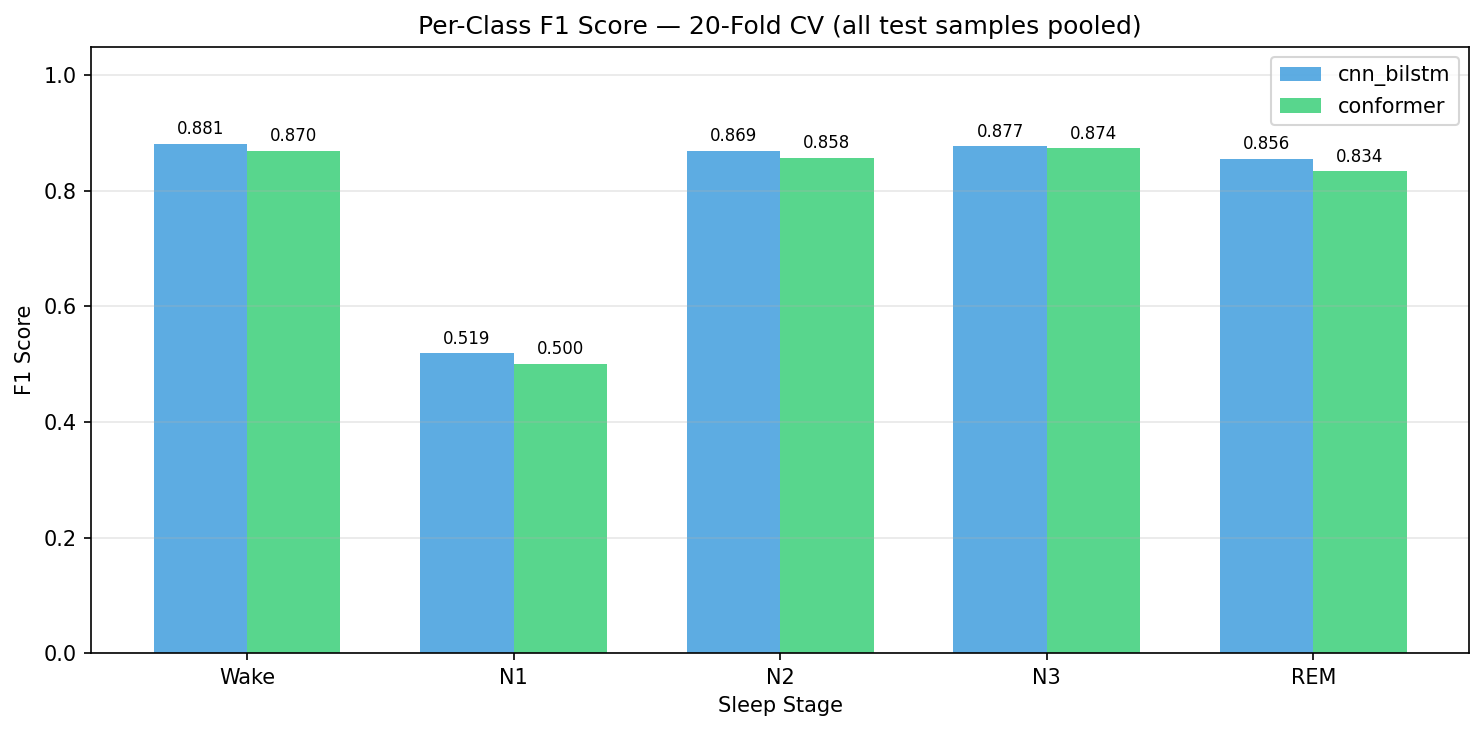
\includegraphics[width=0.72\columnwidth]{cv20_per_class_f1.png}
  \caption{Per-class F1 comparison between CNN+BiLSTM and Conformer across 20-fold LOSO-CV. The BiLSTM leads on all stages except N2 (tied).}
  \label{fig:per_class_f1}
\end{figure}

%--------------------------------------
\subsection{Cross-Validation Stability}
%--------------------------------------

Figure~\ref{fig:boxplots} shows the metric distributions across 20 folds. Both temporal models exhibit high inter-subject variance (std 6.5--7.3\%), reflecting diversity in individual sleep architecture. The BiLSTM shows tighter distributions than the Conformer on all metrics. Fold~11 is a consistent outlier ($\sim$62--64\% accuracy), suggesting atypical sleep patterns for that subject.

Figure~\ref{fig:confusion} presents the pooled confusion matrices. The temporal models show substantially reduced off-diagonal mass in the Wake and REM rows compared to the baseline, confirming that temporal context resolves many Wake$\leftrightarrow$N1 and N1$\leftrightarrow$REM confusions.

\begin{figure}[t]
  \centering
  \begin{subfigure}[b]{0.48\textwidth}
    \centering
    
\includegraphics[width=\textwidth]{../figures/confusion_matrices.png}
    \caption{Baseline (CNN-only)}
  \end{subfigure}
  \hfill
  \begin{subfigure}[b]{0.48\textwidth}
    \centering
    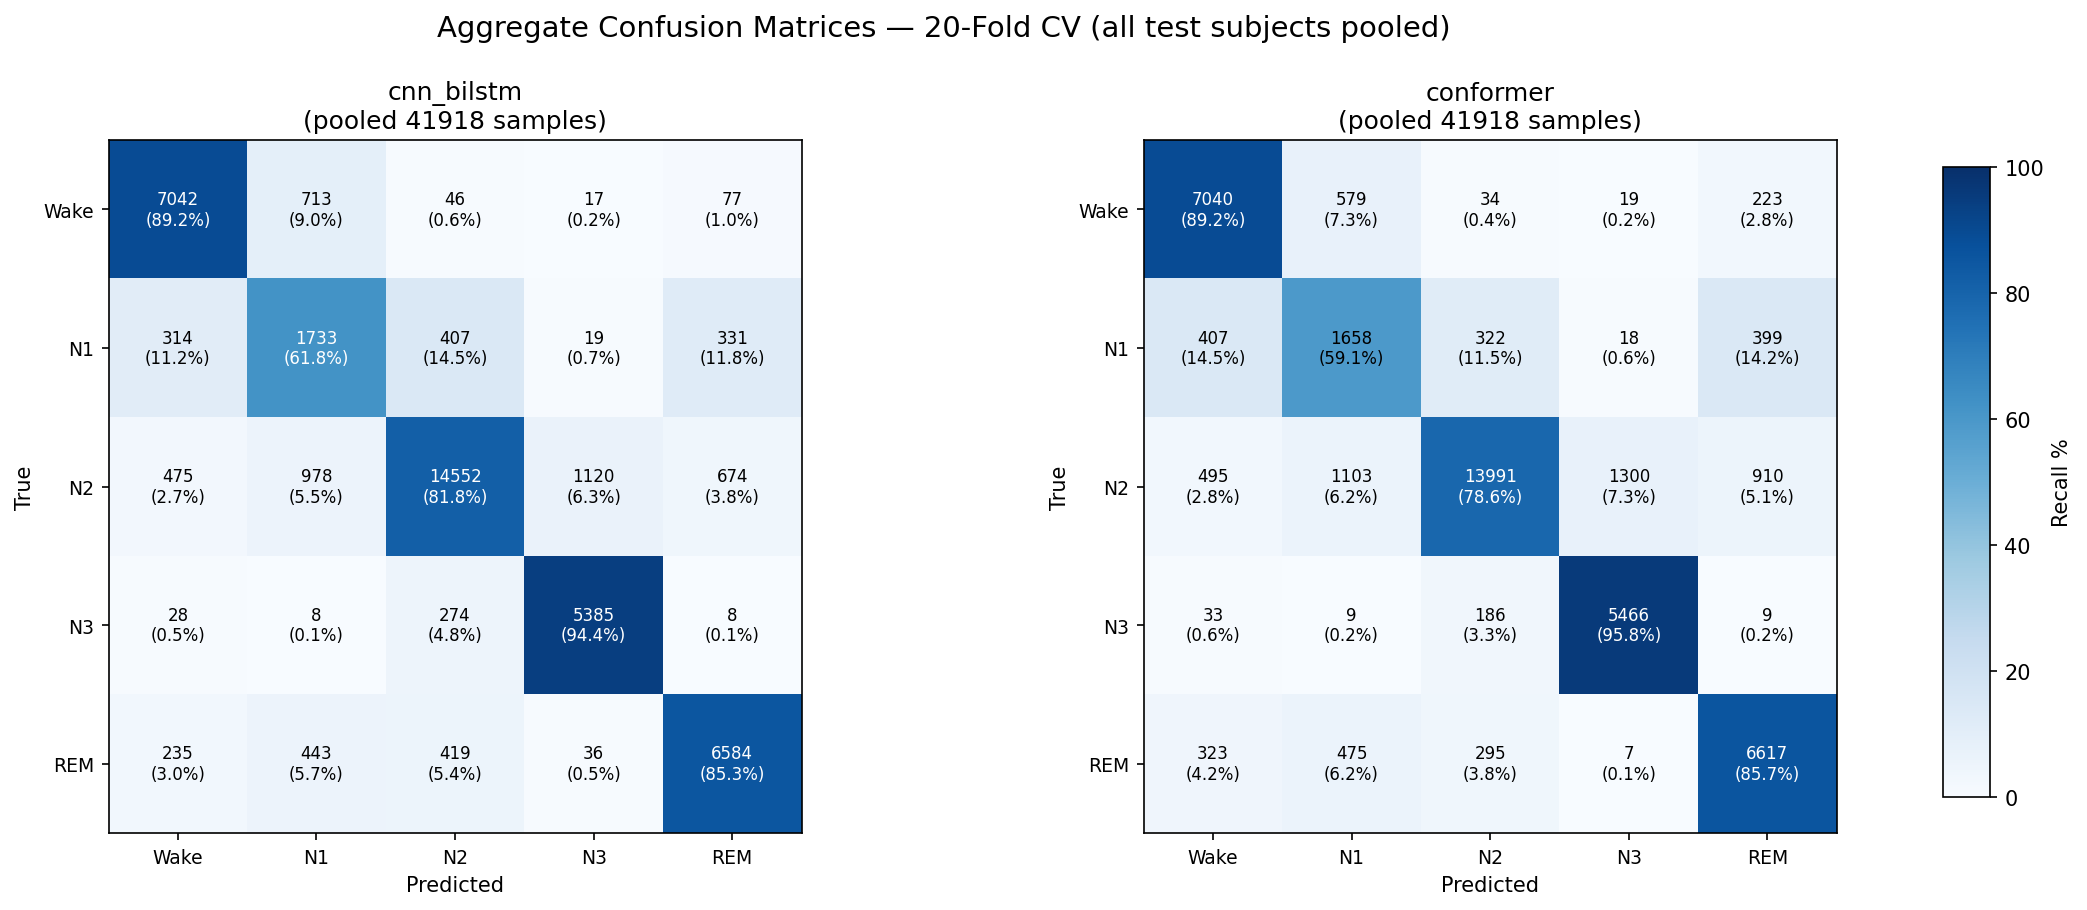
\includegraphics[width=\textwidth]{cv20_confusion_matrices.png}
    \caption{CNN+BiLSTM and Conformer}
  \end{subfigure}
  \caption{Pooled confusion matrices across all 20 folds. (a)~Baseline shows heavy N1 confusion with Wake and N2. (b)~Temporal models substantially reduce off-diagonal errors.}
  \label{fig:confusion}
\end{figure}

\begin{figure}[t]
  \centering
  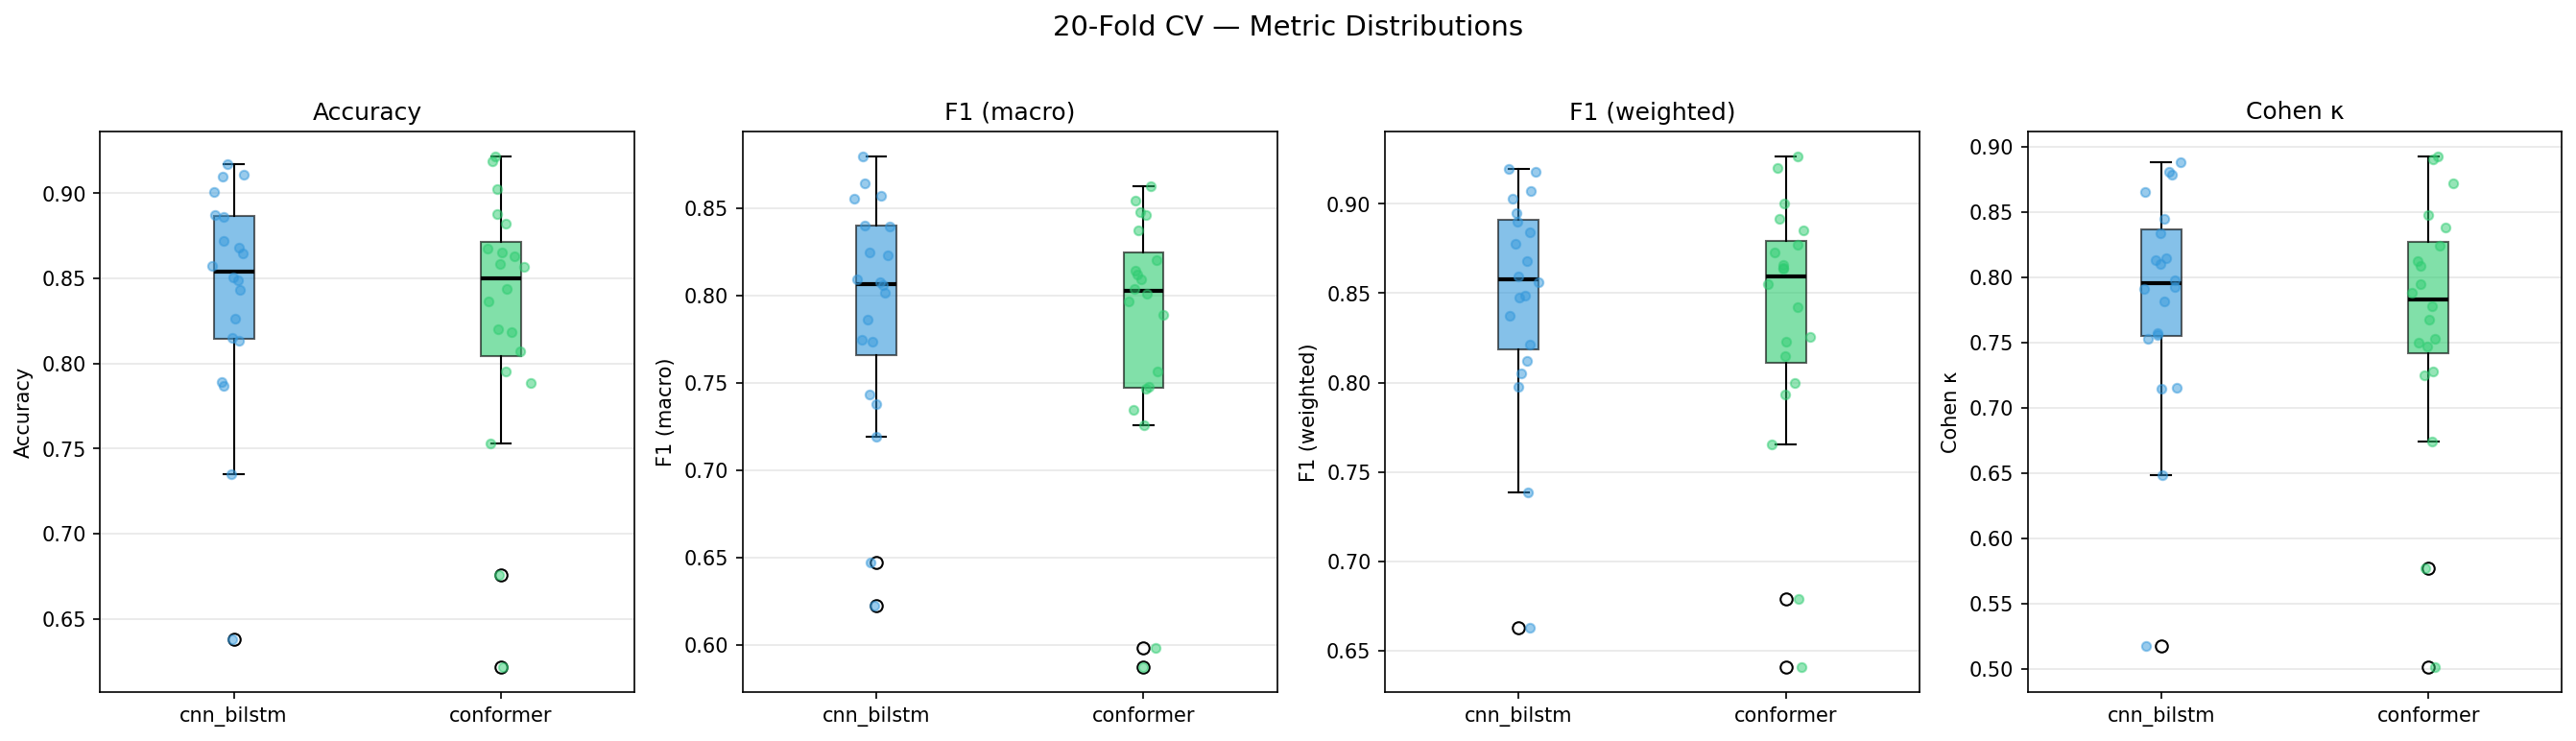
\includegraphics[width=0.80\columnwidth]{cv20_boxplots.png}
  \caption{Distribution of metrics across 20 LOSO-CV folds. The BiLSTM exhibits tighter distributions on all metrics than the Conformer.}
  \label{fig:boxplots}
\end{figure}

%--------------------------------------
\subsection{Clinical Context}
%--------------------------------------

Cohen's $\kappa = 0.778$ for the CNN+BiLSTM places it at the lower bound of human inter-scorer agreement ($\kappa \approx 0.75$--$0.85$)~\cite{Rosenberg2013}. The single-channel requirement (Fpz-Cz only) makes this applicable to consumer-grade wearable devices, though N1 F1 of 0.519 would need improvement for diagnostic use.

For context, published methods on Sleep-EDF report accuracies in the 80--86\% range: DeepSleepNet~\cite{Supratak2017} achieved $\sim$82\% with a similar dual-path CNN+BiLSTM but using a different train/test split; AttnSleep~\cite{Eldele2021} reported $\sim$84.4\% with multi-head attention; and SleepTransformer~\cite{Phan2022} reached $\sim$84--85\% using dual-granularity transformers. Direct comparison is complicated by differences in dataset versions (Sleep-EDF-20 vs.\ Sleep-EDF-78), cross-validation protocols (k-fold vs.\ LOSO), and preprocessing pipelines. Our 20-fold LOSO-CV is among the most rigorous evaluation protocols, as it ensures complete subject independence between training and testing---a requirement for any clinically deployed system. Under this strict protocol, our CNN+BiLSTM's 83.9\% accuracy and $\kappa = 0.778$ are competitive with the state of the art.

%==============================================================================
\section{Discussion}
%==============================================================================

%--------------------------------------
\subsection{Why Does BiLSTM Outperform Conformer?}
%--------------------------------------

The CNN+BiLSTM outperforms the more parameter-rich Conformer across all metrics. We identify four contributing factors:

\textbf{Inductive bias.} The BiLSTM has a strong sequential inductive bias---it processes epochs in temporal order, naturally encoding proximity and direction. Sleep stage transitions are inherently sequential (one does not jump from N3 to REM without passing through lighter stages). The Conformer's self-attention treats all positions as equally accessible and must learn this sequential structure purely from data.

\textbf{Dataset size.} With only 20 subjects and $\sim$42K epochs, the Conformer's larger parameter count (1.34M vs.\ 851K) may lead to overfitting. Attention mechanisms are known to be data-hungry, and 42K training epochs may be insufficient for the Conformer to realize its theoretical advantages over recurrence.

\textbf{Sequence length.} At $L = 11$, the sequence is short enough that the BiLSTM can model dependencies across the full window without vanishing gradients. Self-attention's advantage---direct pairwise connections between distant positions---is less pronounced when all positions are within the LSTM's effective memory horizon.

\textbf{Loss function confound.} The Conformer used focal loss ($\gamma = 1.5$) while the BiLSTM used standard cross-entropy. Although focal loss was intended to improve N1 classification, it may have suboptimally reduced the learning signal for well-classified stages, slightly hurting overall calibration.

%--------------------------------------
\subsection{The N1 Problem}
%--------------------------------------

N1 (light sleep) remains the primary bottleneck across all models, with a best F1 of 0.519. This difficulty reflects fundamental properties of the N1 stage:

\begin{itemize}[nosep, leftmargin=*]
  \item \textbf{Spectral ambiguity:} N1's EEG morphology overlaps with Wake (theta activity in both), N2 (vertex sharp waves resemble K-complexes), and REM (low-amplitude mixed-frequency patterns in both).
  \item \textbf{Brevity:} N1 is a transitional stage lasting only 1--7 minutes, producing few contiguous epochs for learning. It accounts for just 6.6\% of all epochs.
  \item \textbf{Human disagreement:} Even trained scorers exhibit lower inter-rater reliability on N1 than on other stages~\cite{Rosenberg2013}, suggesting an intrinsic limit to automated N1 classification from single-channel EEG.
\end{itemize}

Despite these challenges, temporal context provides a meaningful boost (+17.7\% relative F1). The BiLSTM can leverage transition patterns---e.g., recognizing that an ambiguous epoch between Wake and N2 is likely N1---but cannot fully resolve the underlying spectral ambiguity.

%--------------------------------------
\subsection{Design Decisions}
%--------------------------------------

Several architectural choices merit justification. The \textbf{sequence length} $L = 11$ ($\pm$5 epochs, 5.5 minutes) was chosen to span roughly half a typical sleep cycle transition while keeping GPU memory manageable on Colab T4s (16\,GB). Shorter windows ($L = 5$) miss multi-stage transitions; longer windows ($L = 25$) increase memory quadratically for the Conformer's attention and risk spanning recording boundaries in short recordings.

The \textbf{two-layer BiLSTM} balances expressiveness against overfitting. A single layer suffices for local transitions but struggles with compound patterns (e.g., recognizing the REM-to-Wake transition that signals the end of a sleep cycle). Three or more layers showed no improvement in preliminary experiments and increased training instability.

The \textbf{three Conformer blocks} follow a similar rationale---each block adds $\sim$170K parameters, and we found diminishing returns beyond three. The \textbf{depthwise convolution kernel} $k = 7$ was selected to span approximately $\pm$3 epochs of local context within each Conformer block, complementing the global view provided by self-attention.

%--------------------------------------
\subsection{Computational Efficiency}
%--------------------------------------

Practical deployment requires balancing accuracy against computational cost. The CNN+BiLSTM ($\sim$851K parameters) requires approximately 2.5 hours per fold on a T4 GPU across all three training stages, totaling $\sim$50 GPU-hours for the full 20-fold evaluation. The Conformer ($\sim$1.34M parameters) requires $\sim$3.5 hours per fold ($\sim$70 GPU-hours total) due to the quadratic attention computation. The baseline ($\sim$648K parameters) trains in $\sim$1.5 hours per fold.

At inference, all three models classify an 8-hour recording (960 epochs) in under 10 seconds on a T4 GPU, making them suitable for clinical deployment where overnight results are acceptable. The BiLSTM's advantage is notable: it achieves the best accuracy with 37\% fewer parameters than the Conformer and requires 29\% less training time---a meaningful consideration when retraining on institution-specific data.

%==============================================================================
\section{Limitations and Future Work}
%==============================================================================

\paragraph{Limitations.}
Our study has several limitations: (1)~\textbf{Single EEG channel}---human scorers use EOG and EMG in addition to EEG, providing complementary information our models lack; (2)~\textbf{Small dataset}---20 subjects limits generalization claims, and no external validation on larger datasets (SHHS, MASS) was performed; (3)~\textbf{High subject variance}---some folds achieve $<$65\% accuracy, indicating that certain individuals' sleep patterns are poorly captured by a one-size-fits-all model; (4)~\textbf{No statistical significance testing}---paired tests across folds between BiLSTM and Conformer would strengthen the comparison; (5)~\textbf{Framework confound}---the baseline uses TensorFlow while temporal models use PyTorch, introducing a minor implementation variable.

\paragraph{Future directions.}
Several avenues could address these limitations: (1)~\textbf{Multi-modal inputs}: adding EOG and EMG channels to match clinical practice; (2)~\textbf{Pre-training on larger corpora}: training on SHHS (5,000+ subjects) then fine-tuning on Sleep-EDF, which may unlock the Conformer's capacity advantage; (3)~\textbf{Subject-adaptive fine-tuning}: few-shot personalization or meta-learning (MAML) to reduce inter-subject variance; (4)~\textbf{N1-targeted strategies}: stage-conditional focal loss with higher $\gamma$ for N1, or synthetic N1 generation via EEG augmentation; and (5)~\textbf{Uncertainty quantification}: MC-Dropout confidence estimates for flagging low-confidence epochs in clinical deployment.

%==============================================================================
\section{Conclusion}
%==============================================================================

We presented a systematic comparison of three architectures for automated sleep stage classification, sharing a common multi-scale CNN backbone and differing in temporal modeling. Our results demonstrate that temporal context modeling is the dominant factor for performance, yielding a 3 pp accuracy improvement and 17.7\% relative N1 F1 gain over the CNN-only baseline. The CNN+BiLSTM model achieves $\kappa = 0.778$, approaching the lower bound of human inter-scorer agreement, and outperforms the more complex Conformer---suggesting that recurrent inductive biases are preferable to attention mechanisms on small sequential EEG datasets with $\sim$42K training examples. As wearable EEG devices become more prevalent, lightweight models that operate on single-channel input while achieving near-expert-level agreement will be essential for scalable sleep medicine.

\bibliographystyle{plain}
\bibliography{references}

\end{document}
